\RequirePackage{plautopatch}
\documentclass[14pt,aspectratio=169,xcolor=dvipsnames,table,onlytextwidth,dvipdfmx]{beamer}
\usepackage[utf8]{inputenc}
\usepackage{bxdpx-beamer} % dvipdfmxなので必要

\usetheme{Boadilla}
%Beamerフォント設定
\usefonttheme{professionalfonts}
\usepackage[T1]{fontenc}
\usepackage[deluxe,uplatex]{otf} % 日本語多ウェイト化
\usepackage{mlmodern}  % 太いComputer Modern
% MLmodernのバグを修正: cf. https://tex.stackexchange.com/questions/646333/size-of-integral-symbol-in-section-header-with-mlmodern
\DeclareFontFamily{OMX}{mlmex}{}
\DeclareFontShape{OMX}{mlmex}{m}{n}{%
   <->mlmex10%
   }{}
\usepackage{newtxtext} % 数式以外をTXフォントで上書き
% \usepackage[noalphabet,unicode]{pxchfon}
% \setminchofont{KozMinPro-Regular.otf}% 游明朝Regular
% \setboldminchofont{KozMinPro-Bold.otf}% 游明朝Demibold
% \setgothicfont[0]{BIZ-UDGothicR.ttc}% BIZ UDゴシックR
% \setboldgothicfont[0]{BIZ-UDGothicB.ttc}% BIZ UDゴシックB
\renewcommand{\familydefault}{\sfdefault}  % 英文をサンセリフ体に
\renewcommand{\kanjifamilydefault}{\gtdefault}  % 日本語をゴシック体に
\usefonttheme{structurebold} % タイトル部を太字
\setbeamerfont{alerted text}{series=\bfseries} % Alertを太字
\setbeamerfont{section in toc}{series=\mdseries} % 目次は太字にしない
\setbeamerfont{frametitle}{size=\Large} % フレームタイトル文字サイズ
\setbeamerfont{title}{size=\LARGE} % タイトル文字サイズ
\setbeamerfont{date}{size=\small}  % 日付文字サイズ
\usepackage{bxcoloremoji}

% Babel (日本語の場合のみ・英語の場合は不要)
\uselanguage{japanese}
\languagepath{japanese}
\deftranslation[to=japanese]{Theorem}{定理}
\deftranslation[to=japanese]{Lemma}{補題}
\deftranslation[to=japanese]{Example}{例}
\deftranslation[to=japanese]{Examples}{例}
\deftranslation[to=japanese]{Definition}{定義}
\deftranslation[to=japanese]{Definitions}{定義}
\deftranslation[to=japanese]{Problem}{問題}
\deftranslation[to=japanese]{Solution}{解}
\deftranslation[to=japanese]{Fact}{事実}
\deftranslation[to=japanese]{Proof}{証明}
\deftranslation[to=japanese]{Corollary}{系}
\setbeamertemplate{theorems}[normal font] %日本語の場合，定理内を斜体にしない
% overlay-aware proof environment
\renewenvironment<>{proof}{%
\par
\begin{actionenv}#1%
\structure{(証明)}}
{\qed\end{actionenv}}

%Beamer色設定
\definecolor{UniBlue}{RGB}{0,150,200}
\definecolor{UniGreen}{RGB}{3,175,122}
\definecolor{UniPink}{RGB}{255,128,255}
\definecolor{AlertOrange}{RGB}{255,76,0}
\definecolor{AlmostBlack}{RGB}{38,38,38}
\setbeamercolor{normal text}{fg=AlmostBlack}  % 本文カラー
\setbeamercolor{structure}{fg=UniBlue} % 見出しカラー
\setbeamercolor{block title}{fg=UniBlue!50!black} % ブロック部分タイトルカラー
\setbeamercolor{alerted text}{fg=AlertOrange} % \alert 文字カラー
\setbeamercolor{bibliography entry author}{fg=AlmostBlack} % Bib 文字カラー
\setbeamercolor{bibliography entry note}{fg=AlmostBlack} % Bib 文字カラー
\mode<beamer>{
    \definecolor{BackGroundGray}{RGB}{254,254,254}
    \setbeamercolor{background canvas}{bg=BackGroundGray} % スライドモードのみ背景をわずかにグレーにする
}

%フラットデザイン化
\setbeamertemplate{blocks}[rounded] % Blockの影を消す
\useinnertheme{circles} % 箇条書きをシンプルに
\setbeamertemplate{navigation symbols}{} % ナビゲーションシンボルを消す
\setbeamertemplate{footline}[frame number] % フッターはスライド番号のみ

%タイトルページ
\setbeamertemplate{title page}{%
    \vspace{2.5em}
    {\usebeamerfont{title} \usebeamercolor[fg]{title} \inserttitle \par}
    {\usebeamerfont{subtitle}\usebeamercolor[fg]{subtitle}\insertsubtitle \par}

    \vspace{1.5em}
    \begin{columns}[]
        \begin{column}{.35\linewidth}
        \usebeamerfont{titlegraphic}\inserttitlegraphic\par
        \end{column}
        \begin{column}{.6\linewidth}\setlength\topsep{0pt}
            \begin{flushright}
        \usebeamerfont{author}\insertauthor\par
        \usebeamerfont{institute}\insertinstitute \par
        \vspace{3em}
        \usebeamerfont{date}\insertdate\par
            \end{flushright}
        \end{column}
    \end{columns}
}

%biblatex
% \usepackage[style=ext-authoryear,citestyle=authoryear,natbib=true,giveninits=true,maxbibnames=99,maxcitenames=10,url=false,isbn=false,doi=false,articlein=false]{biblatex}
% \DeclareNameAlias{author}{first-last}
% \addbibresource{shrunk.bib}
% \newcommand{\mkbibbracketscol}[1]{\textcolor{UniBlue}{\scriptsize \mkbibbrackets{#1}}}
% \DeclareCiteCommand{\cite}[\mkbibbracketscol]
%   {\usebibmacro{prenote}}
%   {\usebibmacro{citeindex}%
%    \usebibmacro{cite}}
%   {\multicitedelim}
%   {\usebibmacro{postnote}}
% % \renewcommand{\cite}[1]{\textcolor{UniBlue}{\scriptsize\citep{#1}}}
% \renewcommand*{\finalnamedelim}{\addcomma\addspace} % remove "and" before the last author
% \DeclareDelimFormat{nameyeardelim}{\addspace}
% \setbeamertemplate{bibliography item}{}

% Algorithm系
\usepackage{algorithm}
\usepackage[noend]{algorithmic}
\algsetup{linenosize=\color{fg!50}\footnotesize}
\renewcommand\algorithmicdo{:}
\renewcommand\algorithmicthen{:}
\renewcommand\algorithmicrequire{\textbf{Input:}}
\renewcommand\algorithmicensure{\textbf{Output:}}
\renewcommand\algorithmiccomment[1]{\hfill\textcolor{fg!50}{\footnotesize\textit{// #1}}}

% TikZ
\usepackage{tikz}
\usetikzlibrary{positioning,shapes,arrows,quotes,shapes.callouts,calc,graphs,graphs.standard,fit,backgrounds,perspective,matrix}
\tikzset{point/.style={circle, fill=AlertOrange, inner sep=1pt, text width=1pt}}
\tikzset{bpoint/.style={circle, fill=black, inner sep=1pt, text width=1pt}}
\tikzset{alt/.code args={<#1>#2#3}{\alt<#1>{\pgfkeysalso{#2}}{\pgfkeysalso{#3}}}}
\tikzset{>=latex}
\tikzset{mynodes/.style={circle,white,fill=UniBlue!90,text width=.8em,inner sep=0pt,text centered,font=\footnotesize}}
\tikzset{myedges/.style={thick}}
\tikzset{mypath/.style={ultra thick, draw=#1}, mypath/.default=AlertOrange}
\tikzset{mysubset/.style={draw,#1,dotted,thick,fill=#1!10}, mysubset/.default=UniBlue}
\tikzset{mypath2/.style={ultra thick, dashed, draw=UniGreen}}
\tikzset{graphs/mygraph/.style={nodes={mynodes}, edges={myedges}, empty nodes}}
\tikzset{nomargin/.style={inner sep=0pt, outer sep=0pt}}
%% graph macros
\tikzgraphsset{declare={mybipartite}{%
subgraph I_nm [V={1,2,3,4,5,6}, W={a,b,c,d,e,f}];
1 -- {a,b};
2 -- {b,c,d,e};
3 -- {d,f};
4 -- {e,f};
{5,6} -- f;
}}
\tikzgraphsset{declare={mybipartitedi}{%
subgraph I_nm [V={1,2,3,4,5,6}, W={a,b,c,d,e,f}];
1 -> {a,b};
2 -> {b,c,d,e};
3 -> {d,f};
4 -> {e,f};
{5,6} -> f;
}}
\tikzgraphsset{declare={mybipartite2}{%
subgraph I_nm [V={1,2,3}, W={a,b,c}];
1 -- {a,b}; 2 -- {a,b,c}; 3 -- {a,c};
}} 
% Petersen graph
\tikzgraphsset{declare={Petersen}{%
    subgraph C_n [n=5,name=A, radius=1.5cm]; 
    subgraph I_n [n=5,name=B, radius=.8cm];
    \foreach \i [evaluate={\j=int(mod(\i+2,5)+1);}] in {1,...,5}{
        A \i -- B \i;
        B \i -- B \j;
}}}
% Example graph for Menger's theorem
\tikzgraphsset{declare={menger}{%
    s[at={(-1,0)}, as={$s$}];
    (s) -> 1[at={(0,1)}] -> 2[at={(1,0)}];
    (s) -> 3[at={(0,-1)}] -> 2;
    4[at={(2,1)}] <- 5[at={(2,-1)}];
    {5,6[at={(3,1)}], 7[at={(3,-1)}]} -> t[at={(4,0)}, as={$t$}];
    (s) -> (2);
    (2) -> {(4), (5)};
    {(4),(5)} -> {(6),(7)};
    (6) -> (7);
    1 -> 4;
}} 
\tikzgraphsset{declare={undirected menger}{%
    s[at={(-1,0)}, as={$s$}];
    (s) -- 1[at={(0,1)}] -- 2[at={(1,0)}];
    (s) -- 3[at={(0,-1)}] -- 2;
    4[at={(2,1)}] -- 5[at={(2,-1)}];
    {5,6[at={(3,1)}], 7[at={(3,-1)}]} -- t[at={(4,0)}, as={$t$}];
    (s) -- (2);
    (2) -- {(4), (5)};
    {(4),(5)} -- {(6),(7)};
    (6) -- (7);
    1 -- 4;
}} 

% Appendix
\usepackage{appendixnumberbeamer}

% macros
\newcommand{\R}{\mathbb{R}}
\newcommand{\Z}{\mathbb{Z}}
\newcommand{\be}{\mathbf{e}}
\newcommand{\zeros}{\mathbf{0}}
\newcommand{\ones}{\mathbf{1}}
\newcommand{\bfzero}{\zeros}
\newcommand{\bfone}{\ones}

% \newcommand{\bp}{\mathbf{p}}
\newcommand{\eps}{\varepsilon}
\newcommand{\defiff}{\overset{\text{def}}{\iff}}
\DeclareMathOperator{\poly}{poly}
\DeclareMathOperator{\conv}{conv}
\DeclareMathOperator{\In}{In}
\DeclareMathOperator{\Out}{Out}
\DeclareMathOperator{\val}{val}
\newcommand{\lo}{{\mathrm{lo}}}
\newcommand{\up}{{\mathrm{up}}}
\newcommand{\caI}{\mathcal{I}}
\newcommand{\caB}{\mathcal{B}}
\newcommand{\caC}{\mathcal{C}}
\newcommand{\bM}{\mathbf{M}}
\newcommand{\IO}{\mathrm{IO}}

\usepackage{mathtools}
\DeclarePairedDelimiter{\abs}{\lvert}{\rvert}
\DeclarePairedDelimiter{\norm}{\lVert}{\rVert}
\DeclarePairedDelimiter{\inprod}{\langle}{\rangle}
\usepackage[no-test-for-array]{nicematrix}
\usepackage{diagbox}

\newcommand{\highlightcap}[3][red]{\tikz[baseline=(x.base)]{\node[rectangle,rounded corners,fill=#1!10](x){#2} node[below=0pt of x, color=#1]{#3};}}
\newcommand{\highlight}[2][red]{\tikz[baseline=(x.base)]{\node[rectangle,rounded corners,fill=#1!10](x){#2};}}
\newcommand{\mycite}[2][\footnotesize]{\textcolor{UniBlue}{#1 [#2]}}

%section
% \AtBeginSection[]{
%     \frame[c]{
%         \centering
%         \begin{tikzpicture}
%             \node[white, circle, fill=UniBlue, text centered, text width=.3\linewidth](bullet) {
%                 {\Huge \bf \insertsectionnumber} \\[4em]
%     };
%     \node[text width=.65\linewidth, right=1em of bullet]{%
%         \usebeamerfont{title}\usebeamercolor[fg]{title}\insertsection\par %
%     };
%         \end{tikzpicture}
%     } %目次スライド
% }

%grid
% \usepackage[colorgrid,gridunit=pt,texcoord]{eso-pic}
\newcommand{\postit}[1]{\tikz[overlay, remember picture]{\node[draw,anchor=north east, align=center, rectangle, fill=yellow!10, xshift=-1pt, yshift=-1pt] at (current page.north east) {#1};}}

\usepackage{tcolorbox}
\newtcolorbox{primal}{colback=red!10!white, colframe=red, title=主問題 (P), left=2pt,right=2pt,top=0pt,bottom=0pt}
\newtcolorbox{dual}{colback=blue!10!white, colframe=blue, title=双対問題 (D), left=2pt,right=2pt,top=0pt,bottom=0pt}

% visible on
\usetikzlibrary{overlay-beamer-styles}
\usepackage[normalem]{ulem}
\usepackage{pxrubrica}
\usepackage{booktabs}

\newcommand{\Aphiup}{\textcolor{UniBlue}{A_\varphi^\up}}
\newcommand{\Aphilow}{\textcolor{AlertOrange}{A_\varphi^\lo}}
\newcommand{\bv}{\boldsymbol{v}}
\newcommand{\bx}{\boldsymbol{x}}
\newcommand{\by}{\boldsymbol{y}}
\newcommand{\bz}{\boldsymbol{z}}
\newcommand{\bw}{\boldsymbol{w}}
\newcommand{\bc}{{\boldsymbol c}}
\DeclareMathOperator{\supp}{supp}
\DeclareMathOperator{\argmax}{argmax}
\DeclareMathOperator{\argmin}{argmin}
\DeclareMathOperator{\E}{\mathbb{E}}
\csname endofdump\endcsname
\title{組合せ最適化特論}
\subtitle{第9回（劣モジュラ関数①）}
\author{担当: \textbf{相馬 輔}}
\date{2026/7/14}

\begin{document}
\maketitle
\begin{frame}{}
    \centering\small
    \tikzset{block/.style={rectangle, draw=gray, fill=gray!10, thick, minimum width=3em, minimum height=2em, align=center}}
    \begin{tikzpicture}
        \node[block,] (BM) {重みなし\\二部マッチング};
        \node[block,above=1em of BM.north west, xshift=-2em] (WBM) {重みつき\\二部マッチング};
        \node[block,above=5em of BM.north east, xshift=1em] (NF) {最大流};
        \node[block,above=9em of BM] (MCF) {最小費用流};
        % \node[block,above=1em of NF.north east, xshift=1em] (MC) {最小カット};
        \node[block,right=11em of BM] (MTR) {マトロイド};
        \node[block,above=7em of MTR] (MI) {マトロイド交差};
        \node[block,above=3em of MCF, xshift=7em] (SFM) {劣モジュラ最小化};
        \graph[mygraph]{
            (BM) -> {(WBM), (NF)} -> (MCF);
            {(MTR), (BM)} -> (MI);
            % (NF) -> (MC);
            {(MCF), (MI)} -> (SFM);
        };
        \begin{scope}[on background layer]
            \node[mysubset, fit=(BM) (WBM), "二部マッチング" {below, UniBlue}]{};
            \node[mysubset, AlertOrange, fill=AlertOrange!10, fit=(NF) (MCF), "ネットワークフロー" {above left, AlertOrange}]{};
            \node[mysubset, UniGreen, fill=UniGreen!10, fit=(MTR) (MI), "マトロイド" {below, UniGreen}]{};
        \end{scope}
    \end{tikzpicture}
\end{frame}

\begin{frame}[allowframebreaks]
    \frametitle{各回の内容（予定）} 
    \small
    \begin{enumerate}
        \item (4/23) イントロ+多面体的組合せ論（線形計画法の復習，整数多面体，完全単模行列）
        \item[] \textcolor{gray}{(4/30) 休み}
        \item (5/7) 二部マッチング①（Konig-Egervaryの定理，増加道アルゴリズム，ハンガリー法）
        \item (5/14) 二部マッチング②（最短路問題の復習，逐次最短路法と主双対法，最適性基準からの見方）
        \item (5/21) 最大流① （定式化，最大流最小カット定理，応用例）
        \item (5/28) 最大流②（残余ネットワーク，Ford--Fulkerson法，Edmonds--Karpのアルゴリズム）+ 最小費用流①（定式化，輸送問題，最大流との関係）
        \item[] \textcolor{gray}{(6/4) 休み}
        % \item[] \sout{(12/11) 最小カット（永持茨木のアルゴリズム，Kargerのアルゴリズム）}
        \item (6/11) 最小費用流②（逐次最短路法，容量スケーリング法）
        \item[] \textcolor{gray}{(6/18) 休み}
        \item[] \textcolor{gray}{(6/25) 休み}
        \item (7/2) マトロイド（定義と公理系，貪欲法，マトロイド多面体） 
        \item (7/9) 独立マッチング・マトロイド交差 （定義，応用例，Edmondsの最大最小定理，増加道アルゴリズム）
        \item (7/16) 劣モジュラ関数①（諸例，劣モジュラ基多面体，Lov\'asz拡張，劣モジュラ最小化）
        \item[] \textcolor{gray}{(7/23) 休み}
        \item (7/30) 劣モジュラ関数②（劣モジュラ最大化，近似アルゴリズム，貪欲法）
        \item (どこか) 精選トピック①
        \item (どこか) 精選トピック②
        \item (どこか) 精選トピック③
    \end{enumerate}

    \bigskip
    \begin{itemize}
        \item レポート課題を6月と期末に出す予定
        \item 精選トピックの日時は今後調整 
    \end{itemize}
\end{frame}

\begin{frame}<1>[label=outline]{目次}
\begin{tikzpicture}
    \tikzstyle{block} = [rectangle, text width=\textwidth, rounded corners, minimum height=4em]
    \tikzstyle{line} = [draw, -latex]

    \node[block,alt={<1,3->{fill=cyan!10}{fill=red!10}}] (combopt) {
        \begin{columns}
            \begin{column}{0.5\linewidth}
        \textbf{1. 劣モジュラ関数}
            \end{column}
            \begin{column}{0.4\linewidth}
                \small
                \structure{・} 定義 \\
                \structure{・} 諸例
            \end{column}
        \end{columns}
    };
    \node[block,alt={<1-2,4->{fill=cyan!10}{fill=red!10}}, below=.5em of combopt] (LP) {
        \begin{columns}
            \begin{column}{0.5\linewidth}
        \textbf{2. 基多面体とLov\'asz拡張}
            \end{column}
            \begin{column}{0.4\linewidth}
                \small
                \structure{・} 基多面体 \\
                \structure{・} 貪欲法 \\
                \structure{・} Lov\'asz拡張
            \end{column}
        \end{columns}
    };
    \node[block,alt={<1-3,5->{fill=cyan!10}{fill=red!10}}, below=.5em of LP] {
        \begin{columns}
            \begin{column}{0.5\linewidth}
        \textbf{3. 最小ノルム点法}
            \end{column}
            \begin{column}{0.4\linewidth}
                \small
                \structure{・} パラメトリック劣モジュラ最小化 \\
                \structure{・} $L_2$正則化Lov\'asz拡張最小化 \\
                \structure{・} 最小ノルム点法
            \end{column}
        \end{columns}
    };
\end{tikzpicture}%
\end{frame}

%%%%%%%%%%%%%%%%%%%%%%%%%%%%%%%%%%%%%%%%%%%%%
\section{劣モジュラ関数}
\againframe<2|handout:0>{outline}
%%%%%%%%%%%%%%%%%%%%%%%%%%%%%%%%%%%%%%%%%%%%%
\begin{frame}{劣モジュラ関数}
    \begin{block}{}
        $f : 2^V \to \R$ が\alert{劣モジュラ関数} \\
        $\defiff f(X) + f(Y) \geq f(X\cup Y) + f(X \cap Y)$ \hfill ($\forall X, Y \subseteq V$) \\
        $\iff$
        $\forall X \subseteq \forall Y \subseteq V$, $\forall a \in V\setminus Y$,
        \setlength{\abovedisplayskip}{0pt}
        \[
            \highlightcap[AlertOrange]{$f(X \cup a) - f(X)$}{\small 小さい集合の増分} \geq \highlightcap[blue]{$f(Y\cup a) - f(Y)$}{\small 大きい集合の増分} 
            \qquad \text{\alert{限界効用逓減性}}
        \]
    \end{block}

    \vfill
    % \begin{center}
    %     \includegraphics[width=.5\linewidth]{figs/dimreturn2.png}
    % \end{center}
    \begin{center}
    \huge
    \begin{tikzpicture}
        \node[inner sep=0pt] (e1) {\coloremoji{🍜}};
        \node[below left=.1em of e1,inner sep=0pt] (e2) {\coloremoji{🍰}};
        \node[below right=.1em of e1,inner sep=0pt] (e3) {\coloremoji{🍔}};
        \node[right=3em of e3,inner sep=0pt,"\normalsize $a$" above] {\coloremoji{🍟}};
        \begin{scope}[on background layer]
            \node[draw,Blue,fill=blue!5,dotted,very thick,fit=(e1) (e2) (e3),"\normalsize $Y$" {blue,left}] {};
            \node[draw,AlertOrange,fill=AlertOrange!20,dotted,very thick,fit=(e3),inner sep=3pt,"\normalsize $X$" {AlertOrange,above}] {};
        \end{scope}
    \end{tikzpicture}
\end{center}
\end{frame}

\begin{frame}{劣モジュラ関数}
    \begin{itemize}
        \setlength{\itemsep}{1em}
        \item $f_1, f_2$ 劣モジュラ関数, $\alpha_1, \alpha_2 \geq 0$ \\
         $\implies$ $\alpha_1 f_1 + \alpha_2 f_2$も劣モジュラ関数

        \item 特に，
    \[
        f(X) + f(Y) = f(X \cup Y) + f(X \cap Y) 
    \]
    が成り立つ場合，$f$を\alert{モジュラ関数}という．\\
    {\footnotesize 例: $f(X) = |X|$や，重み$w: E \to \R$に対する$f(X) = w(X)$など．}


        \item $-f$が劣モジュラである関数を\alert{優モジュラ関数}という．すなわち，
    \[
        f(X) + f(Y) \leq f(X \cup Y) + f(X \cap Y) 
    \]
        が成り立つ関数．
    \end{itemize}
    
    \bigskip
\end{frame}



\begin{frame}{例1: 被覆関数 (coverage function)}
    \begin{columns}
        \begin{column}{.55\linewidth}
    $G = (V^+, V^-; E)$ ... 2部グラフ \\
    \begin{block}{}
    \[
        f(X) = |\Gamma(X)|
    \]
    {\small ($\Gamma(X)$: $X \subseteq V^+$の隣接頂点)}
    \end{block}
        \end{column}
        \begin{column}{.4\linewidth}
            \small
            \begin{tikzpicture}
                \graph[grow right=4em,mygraph]{
                    subgraph I_nm[V={1,2,3,4}, W={a,b,c,d}];
                    1 -- {a, b};
                    2 -- {b, c};
                    3 -- {c};
                    4 -- {a, d};
                };
                \begin{scope}[on background layer]
                    \node[draw,UniBlue,fill=UniBlue!10,rectangle,dotted,thick,fit=(1) (2),"$X$" {UniBlue,left}]{};
                    \node[draw,AlertOrange,fill=AlertOrange!10,rectangle,dotted,thick,fit=(a) (b) (c),"$\Gamma(X)$" {AlertOrange,right}]{};
                \end{scope}
            \end{tikzpicture}
        \end{column}
    \end{columns}

    \vfill\pause
    \structure{重み付き版}
    \begin{block}{}
    $w: V^- \to \R_+$: 非負重み
    \[
        f(X) = w(\Gamma(X))
    \]
    \end{block}
\end{frame}

\begin{frame}{例2: 凹関数と線形関数の合成}
    \begin{columns}
        \begin{column}{.55\linewidth}
            $V = \{1, \dots, n\}$ \\
    $\varphi : [0, +\infty) \to \R$ ... 凹関数 \\
    $w: V \to \R_+$ ... 非負重み

    \begin{block}{}
    \[
    f(X) = \varphi(w(X))
    \]
    \end{block}
        \end{column}
        \begin{column}{.4\linewidth}
            \pgfmathdeclarefunction{myfunc}{1}{%
                \pgfmathparse{%
                2.5*(1-exp(-####1))}%
            }
            \begin{tikzpicture}[>=latex,scale=1.2]
                \draw[->] (0,0) -- (4,0);
                \draw[->] (0,0) -- (0,3);
                \draw[domain=0:4,smooth,variable=\x,UniBlue,thick] plot ({\x},{myfunc(\x)});
                \coordinate(a) at (0.5,{myfunc(0.5)});
                \coordinate(b) at (1.5,{myfunc(1.5)});
                \coordinate(c) at (2,{myfunc(2)});
                \coordinate(d) at (3,{myfunc(3)});

                \foreach \x in {a,b,c,d}
                    \draw[dotted,thick] (\x -| 0,0) -- (\x) -- (\x |- 0,0);

                \draw[UniBlue,->,thick] (a |- 0,0) -- (b |- 0,0);
                \draw[UniBlue,->,thick] (c |- 0,0) -- (d |- 0,0);
                \draw[AlertOrange,<->,thick] (a -| 0,0) -- (b -| 0,0);
                \draw[AlertOrange,<->,thick] (c -| 0,0) -- (d -| 0,0);
            \end{tikzpicture}
        \end{column}
    \end{columns}
\end{frame}


\begin{frame}{例3: グラフのカット関数}
    $G = (V, A)$ ... 有向グラフ \\
    $u: A \to \R_+$ ... 非負枝容量
    \begin{block}{}
        \[
            f(X) = u(\Out(X)) \quad (X \subseteq V) 
        \]
    \end{block}
\end{frame}

\begin{frame}{限界効用逓減性}
    \small
    \structure{記号} $f(a \mid X) := f(X \cup a) - f(X)$ ($X \subseteq V$, $a \in V\setminus X$ \\ {\color{gray}\dotfill $X$に$a$を追加したときの増分}
    \begin{lemma}
        $f: 2^V \to \R$が劣モジュラ $\iff$ $f(a \mid X) \geq f(a \mid Y)$ ($\forall X \subseteq \forall Y \subseteq V$, $\forall a \in V\setminus Y$) \\
    \end{lemma}
    \structure{(証明)}
    \textbf{[$\implies$]} 
    $X + a$と$Y$に対し，劣モジュラ性を使うと
    \begin{align*}
        f(X + a) + f(Y) &\geq f((X + a) \cup Y) + f((X + a) \cap Y) \\
        &= f(Y + a) + f(X \cap Y).
    \end{align*}
    移項すると限界効用逓減性が出る．
\end{frame}

\begin{frame}{証明の続き}
    \small
    \begin{columns}[T]
    \begin{column}{.8\textwidth}
    \textbf{[$\impliedby$]}
 任意の$X, Y \subseteq V$を取る．
$Y \setminus X = \emptyset$の場合は自明なので，$Y \setminus X \neq \emptyset$と仮定して良い．
$Y \setminus X = \{e_1, \dots, e_\ell\}$ ($\ell \geq 1$) とおく．
\[
S_i = (X \cap Y)\cup\{e_1, \dots, e_i\}, \quad T_i = X \cup \{e_1, \dots, e_i\} 
\]
($i=1, \dots, \ell$) とする．
また，$S_0 = X\cap Y$, $T_0 = X$と定義する．
    \end{column}
    \begin{column}{.2\textwidth}
    \centering
        \tikz{
            \node[circle, fill=UniBlue, opacity=.3, minimum size=1.8cm] (B1) at (0,0) {};
            \node[circle, fill=AlertOrange, opacity=.3, minimum size=2cm] (B2) at (1,0) {};
            \node[point,fill=AlertOrange,"$e_1$" right] (j) at ([xshift=.3cm, yshift=.4cm] B2.base) {};
            \node[point,fill=AlertOrange,"$e_2$" right] (k) at ([xshift=.4cm, yshift=0cm] B2.base) {};
            \node[point,fill=AlertOrange,"$e_3$" right] (l) at ([xshift=.3cm, yshift=-.4cm] B2.base) {};
            \node[UniBlue, above=1pt of B1, xshift=-.4cm] {$X$};
            \node[AlertOrange, above=1pt of B2, xshift=+.4cm] {$Y$};
        }
    \end{column}
    \end{columns}

\pause
\bigskip
このとき，$S_{i-1} \subseteq T_{i-1}$, $e_i \notin T_{i-1}$ ($\forall i$)である．
限界効用逓減性より
\[
    f(S_{i-1} \cup  e_ i ) - f(S_{i-1}) \geq f(T_{i-1} \cup  e_i ) - f(T_{i-1}) \qquad (i=1,\dots,\ell)
\]
この式を$i$に対して足し上げると
\[
    f(S_\ell) - f(S_0) \geq f(T_\ell) - f(T_0).
\]
$S_\ell=Y$, $S_0=X\cap Y$, $T_\ell=X\cup Y$, $T_0 = X$なので，劣モジュラ性が得られる．\qed


\end{frame}

\begin{frame}{劣モジュラ関数最小化}
    $f: 2^V \to \R$ 劣モジュラ関数, $f(\emptyset) = 0$

    \begin{block}{劣モジュラ関数最小化}
        \[
            \text{minimize} \quad f(X) \quad \text{subject to} \quad X \subseteq V 
        \]
    \end{block}

    \vfill
    \small
    \begin{overlayarea}{\textwidth}{9em}
    \onslide*<1>{
    \structure{例:}
    \begin{itemize}
        \item K\H{o}nig--Egerv\'ary: $\displaystyle \max_{M: \text{マッチング}} |M| = \min_{X \subseteq V^+} |V^+ \setminus X| + |\Gamma(X)|$
        \item 最大流最小カット定理: $\displaystyle \max_{\varphi: \text{$s$--$t$フロー}} \val(\varphi) = \min_{s \in X \subseteq V - t} u(\Out(X))$
        \item 独立マッチング: $\displaystyle \max_{M: \text{独立マッチング}} |M| = \min_{X \subseteq V^+} r^+(V^+ \setminus X) + r^-(\Gamma(X))$
    \end{itemize}
    }
    \onslide*<2>{
    組合せ的なもの・連続最適化によるものなど様々な技法がある
    \begin{itemize}
        \item Gr\"otschel--Lov\'asz--Schrijver (1981): \textbf{Lov\'asz拡張} + 楕円体法
        \item 岩田--Fleischer--藤重 (2000, 2001), Schrijver (2000): 組合せ的
        \item Lee--Sidford--Wong (2015): 切除平面法
    \end{itemize}
    }
    \end{overlayarea}
\end{frame}

%%%%%%%%%%%%%%%%%%%%%%%%%%%%%%%%%%%%%%%%%%%%%
\section{基多面体とLov\'asz拡張}
\againframe<3|handout:0>{outline}
%%%%%%%%%%%%%%%%%%%%%%%%%%%%%%%%%%%%%%%%%%%%%
\begin{frame}{基多面体}
    \setlength{\abovedisplayskip}{0pt}
    \begin{definition}
        \begin{align*}
            P(f) &:= \{ x \in \R^V : x(X) \leq f(X) \; (\forall X \subseteq V)\} \quad \text{劣モジュラ多面体} \\
            B(f) &:= \{ x \in P(f) : x(V) = f(V)\} \quad \text{基多面体}
        \end{align*}
    \end{definition}

    \vfill
    cf. マトロイド多面体・基多面体（第7回）
        \begin{align*}
            P(\bM) &:= \{ x \in \R^E : x(X) \leq r(X) \; (\forall X \subseteq E)\} \\
            B(\bM) &:= \{ x \in P(\bM) : x(E) = r(E)\} 
        \end{align*}
\end{frame}

\begin{frame}{基多面体上の線形最適化}
    \small
    $w \in \R^V$
    \begin{block}{}
        \[
            \text{maximize} \quad w^\top x \quad \text{subject to} \quad x \in B(f)
        \]
    \end{block}

    \bigskip
    \begin{block}{貪欲法}
    \begin{algorithmic}[1]
        \STATE $V$の要素を$w$の降順に並べる: $w(v_1) \geq \dots \geq w(v_n)$ ($n = \abs{V}$).
        \STATE $x \in \R^V$を次のように定める: $x(v_i) := f(v_i \mid \{v_1, \dots, v_{i-1}\})$ ($i = 1, \dots, n$)
    \end{algorithmic}
    \end{block}
    cf. マトロイドの最小重み基に対する貪欲法

    \bigskip
    \begin{theorem}
        貪欲法における$x$は基多面体上の線形最適化の最適解である．
    \end{theorem}
\end{frame}

\begin{frame}{定理の証明 (1/3)}
    \small
    \textbf{[$x \in B(f)$であること]} まず，$\forall X \subseteq V$に対し，$x(X) \leq f(X)$を示す．
    \begin{align*}
        x(X) &= \sum_{i: v_i \in X} f(v_i \mid \{v_1, \dots, v_{i-1}\}) \\
        &\leq \sum_{i: v_i \in X} f(v_i \mid \{v_1, \dots, v_{i-1}\} \cap X) \\
        &= f(X) - f(\emptyset) = f(X)
    \end{align*}
    また，定義から
    \[
        x(V) = \sum_{i=1}^n f(v_i \mid \{v_1, \dots, v_{i-1}\}) = f(V) - f(\emptyset) = f(V). 
    \]
    ∴$x \in B(f)$.
\end{frame}

\begin{frame}{定理の証明 (2/3)}
    \small
    \textbf{[$x$が最適であること]} 
    $y \in B(f)$を任意に取る．$w^\top x - w^\top y \geq 0$を示したい．
    \begin{align*}
        w^\top x - w^\top y 
        &= \sum_{i=1}^n (x(v_i) - y(v_i)) w(v_i) 
    \end{align*}
    \pause
    \setlength{\abovedisplayskip}{0pt}
    {\footnotesize
    \begin{block}{Abel変形}
        \[
            \sum_{i=1}^n a_i b_i = S_n b_n - \sum_{i=1}^{n-1} S_i (b_{i+1} - b_i) \quad \text{ここで$S_i := \sum_{j \leq i} a_j$} 
        \] 
    \end{block}
    }
    \pause
    \begin{align*}
        w^\top x - w^\top y 
        &= S_n w(v_n) - \sum_{i=1}^{n-1} S_i (w(v_{i+1}) - w(v_i)) 
    \end{align*}
    よって，$S_i \geq 0$ ($i = 1, \dots, n-1$)を示せばよい．
\end{frame}

\begin{frame}{定理の証明 (3/3)}
    \small
    \structure{Claim.} $S_i \geq 0$ ($i = 1, \dots, n-1$) \\[1em]
    \structure{(∵)}
    \begin{align*}
        S_i &= \sum_{j=1}^i (x(v_j) - y(v_j)) \\
        &= \sum_{j=1}^i f(v_j \mid \{v_1, \dots, v_{j-1}\}) - y(\{v_1, \dots, v_i\}) \\
        &= f(\{v_1, \dots, v_i\}) - y(\{v_1, \dots, v_i\}) \geq 0 \tag{$y \in B(f)$}
    \end{align*}
    \qed
\end{frame}

\begin{frame}{Lov\'asz拡張}
    \begin{definition}
        $\hat f: \R^V \to \R$, $\hat f(w) := \max_{x \in B(f)} w^\top x$ を\alert{Lov\'asz拡張}という．
    \end{definition}

    \bigskip
    貪欲法の解を代入すると，
    \begin{align*}
        \hat f(w) 
        &= \sum_{i=1}^n w(v_i) f(v_i \mid \{v_1, \dots, v_{i-1}\})  \\
        &= f(V) w(v_n) + \sum_{i=1}^{n-1} f(\{v_1, \dots, v_i\}) (w(v_i) - w(v_{i+1}))
    \end{align*}
\end{frame}


\begin{frame}{Lov\'asz拡張}
    \begin{columns}
    \begin{column}{.7\textwidth}
    {\small
    \begin{block}{}
        \setlength{\abovedisplayskip}{0pt}
    \begin{align*}
        \hat f(w) 
        &= f(V) w(v_n) + \sum_{i=1}^{n-1} f(\{v_1, \dots, v_i\}) (w(v_i) - w(v_{i+1}))
    \end{align*}
    \end{block}
    }
    特に$w \in [0,1]^V$に限ると，次式になる:
    \begin{block}{}
        \[
            \hat f(w) = \E_{\theta \sim [0,1]}[f(\{w \geq \theta\})]
        \]
    \end{block}
    \small ここで， $\theta \sim [0,1]$は一様分布に従う確率変数．また，略記
    \[
        \{w \geq \theta \} := \{v \in V : w(v) \geq \theta\}
    \]
    を用いた．
    \end{column}
    \begin{column}{.3\textwidth}
        \centering
        \begin{tikzpicture}[xscale=.5, yscale=2]
            \draw[very thick,->] (0,0) -- (5.5,0);
            \draw[very thick,->] (0,0) -- (0,1.5) node[left]{$w$};
            \begin{scope}[on background layer]
                \draw[rectangle, fill=AlertOrange!10] (0,0) rectangle ++(1, 1);
                \draw[rectangle, fill=AlertOrange!10] (1,0) rectangle ++(1,.9);
                \draw[rectangle] (2,0) rectangle ++(1,.6);
                \draw[rectangle] (4,0) rectangle ++(1,.1);
            \end{scope}
            \draw[AlertOrange, very thick, dotted] (0,.7) node[left]{$\theta$} -- ++(5.5,0);
            \foreach \i in {1,2,3}{
                \node[below] at ($(\i,0)+(-.5,0)$) {$v_\i$};
            }
            \draw[AlertOrange, thick, <->] (0,-.3) -- ++(2,0) node[midway,below]{$\{w \geq \theta\}$};
        \end{tikzpicture}
    \end{column}
    \end{columns}
\end{frame}

\begin{frame}{Lov\'asz拡張の例}
    \centering
    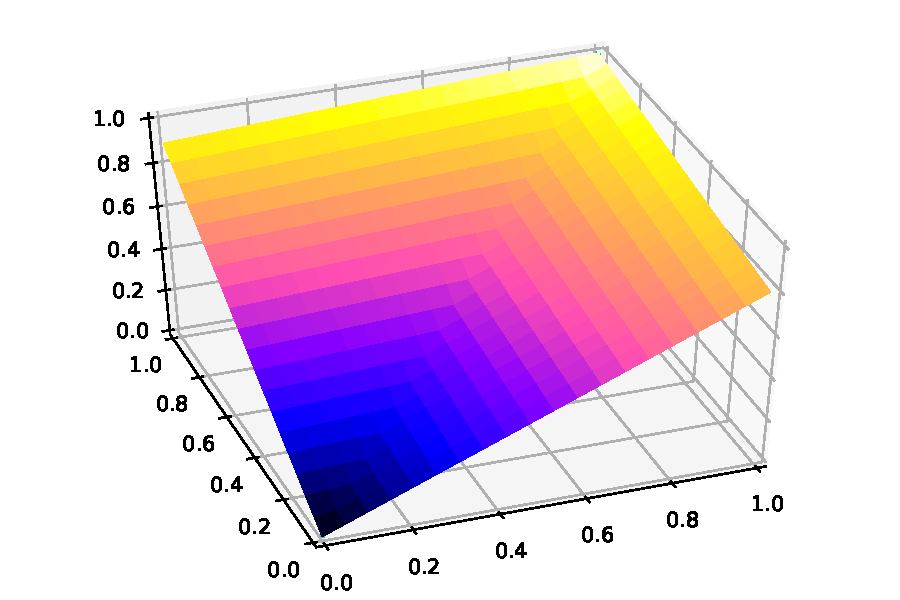
\includegraphics[height=.9\textheight]{figs/Lovext.pdf}
\end{frame}

\begin{frame}{Lov\'asz拡張の性質}
    \small
    \begin{columns}
    \begin{column}{.47\textwidth}
    \begin{lemma}
        \begin{enumerate}
            \item $\hat f$は凸関数．
            \item $\hat f(\ones_X) = f(X)$ ($X \subseteq V$)
            \item $\displaystyle \min_{w \in [0,1]^V} \hat f(w) = \min_{X \subseteq X} f(X)$
        \end{enumerate}
    \end{lemma}
    \end{column}
    \begin{column}{.5\textwidth}
        これらより，凸関数$\hat f$の最小化で劣モジュラ関数$f$の最小化ができる． \\
        \hfill $\longrightarrow$ 楕円体法\mycite{GLS81}
    \end{column}
    \end{columns}
    \pause
    \vfill
    \begin{proof}
        \begin{itemize}
            \item[①] $\hat f(w) = \max_{x \in B(f)} w^\top x$であり，一般に複数の線形関数の最大値は凸関数．
            \item[②] 期待値の式から自明．

            \item[③] ②より$\text{左辺} \leq \text{右辺}$．一方，$w \in [0,1]^V$に対し$\hat f(w) = \E[f(\dots)] \geq \text{右辺}$.
        \end{itemize}
    \end{proof}
\end{frame}


%%%%%%%%%%%%%%%%%%%%%%%%%%%%%%%%%%%%%%%%%%%%%
\section{最小ノルム点法}
\againframe<4|handout:0>{outline}
%%%%%%%%%%%%%%%%%%%%%%%%%%%%%%%%%%%%%%%%%%%%%
\begin{frame}{最小ノルム点法}
    \centering
    \tikzset{block/.style={fill=cyan!10,rectangle,rounded corners,align=center}}
    \begin{tikzpicture}
        \node[block](SFMa){\textbf{パラメトリック劣モ最小化} \\
        $\displaystyle \min_{X \subseteq V} f(X) + \alpha \abs{X}$ \quad (SFM$_\alpha$)};
        \node[block, below=5em of SFMa](P){\textbf{$L_2$正則化Lov\'asz拡張最小化} \\
        $\displaystyle \min_{w \in \R^V} \hat f(w) + \frac{1}{2} \norm{w}^2$ \quad (P)};
        \node[block, right=10em of P](MN){\textbf{最小ノルム点} \\
        $\displaystyle \min_{x \in B(f)} \norm{x}^2$};
        \node[blue, above=1em of MN, align=center, font=\footnotesize](FW){Wolfeのアルゴリズム \\ (\textbf{藤重--Wolfe法}) \\ 実用上最速};
        \graph[mygraph, edges={gray}]{
            (SFMa) <->["定理"] (P);
            (P) <->["等価 ($w^* = -x^*$)" above] (MN);
            (FW) --[blue, dotted] (MN);
        };
    \end{tikzpicture}
\end{frame}

\begin{frame}{パラメトリック劣モジュラ最小化}
    \small
    \begin{block}{}
        \[
        \min_{X \subseteq V} f(X) + \alpha \abs{X} \qquad (\text{SFM}_\alpha)
        \]
    \end{block}
    パラメータ$\alpha \in \R$は動く

    \bigskip
    \structure{Claim.} $A_\alpha$: (SFM$_\alpha$)の最適解とすると，$\alpha < \beta \implies A_\alpha \supseteq A_\beta$. \\[1em]

    \onslide<2->{\footnotesize 
    \structure{(∵)} $A_\alpha, A_\beta$がそれぞれ最適解であることから，
    \begin{align*}
        f(A_\alpha) + \alpha \abs{A_\alpha} &\leq f(A_\alpha \cup A_\beta) + \alpha \abs{A_\alpha \cup A_\beta}, \\
        f(A_\beta) + \beta \abs{A_\beta} &\leq f(A_\alpha \cap A_\beta) + \beta \abs{A_\alpha \cap A_\beta}.
    \end{align*}
    足して，移項すると
    \begin{align*}
        (\beta - \alpha) \abs{A_\beta \setminus A_\alpha} \leq f(A_\alpha \cup A_\beta) + f(A_\alpha \cap A_\beta) - f(A_\alpha) - f(A_\beta) \leq 0
    \end{align*}
    $\beta - \alpha > 0$より，$\abs{A_\beta \setminus A_\alpha} = 0$. \qed
    }
\end{frame}

\begin{frame}{$L_2$正則化Lov\'asz拡張最小化}
    \small
    \begin{block}{}
        \[ \min_{w \in \R^V} \hat f(w) + \frac{1}{2} \norm{w}^2 \qquad \text{(P)}\]
    \end{block}
    \vfill
    $A_\alpha$: (SFM$_\alpha$)の最適解．
    \begin{theorem}
        $w \in \R^V$を$w(v) := \sup\{\alpha : v \in A_\alpha\}$と定めると，$w$は(P)の一意な最適解である．
    \end{theorem}

    \vfill
    \structure{系:}
    $w^*$: (P)の（一意）最適解とする．
    \begin{itemize}
        \item $\{w^* \geq \alpha\}$は(SFM$_\alpha$)の最適解 \\ \alert{(SFM$_\alpha$)の全ての最適解が得られる！}
        \item 特に，$\alpha = 0$とすると，次が得られる: \\ 
        $\{w^* \geq 0\}$は劣モジュラ最小化$\displaystyle \min_{X \subseteq V}f(X)$の最適解
    \end{itemize}
\end{frame}

\begin{frame}{定理の証明 (1/2)}
    \small

    \structure{Claim.} ほとんどすべての$\alpha$について$A_\alpha = \{w \geq \alpha\}$. \\
    \onslide<2->{
    \structure{(∵)}
        $w$の定義から，
        \begin{itemize}
            \item $w(v) < \alpha \implies v \notin A_\alpha$. \hfill ∴$A_\alpha \subseteq \{w \geq \alpha\}$.
            \item $w(v) > \alpha \implies \alpha < \exists \beta < w(v)$ s.t. $v \in A_\beta$. \\ 
            Claim「$\alpha < \beta \implies A_\alpha \supseteq A_\beta$」より，$v \in A_\alpha$.
            \hfill ∴$\{w > \alpha \} \subseteq A_\alpha$.
        \end{itemize}
        よって，$\{w > \alpha\} \subseteq A_\alpha \subseteq \{w \geq \alpha\}$が成り立つ． \qed
    }
    \vfill
    \structure{Claim.} $\hat f(w) + \frac{1}{2} \norm{w}^2 \leq \hat f(w') + \frac{1}{2} \norm{w'}^2$ ($\forall w' \in \R^V$) 
\end{frame}

\begin{frame}{定理の証明 (2/2)}
    \small
    \structure{(∵)} 任意の$w' \in \R^V$に対し，$\beta < 0$を十分小さく取ると，
    \footnotesize
    \begin{align*}
        \hat f(w) + \frac{1}{2} \norm{w}^2
        &= \int_\beta^{+\infty} f(\{w \ge \alpha\}) d\alpha + \beta f(V) 
        + \sum_{v \in V} \bigg[ \int_\beta^{w(v)} \alpha d\alpha + \frac{1}{2} \beta^2 \bigg] \\
        &= \text{const.} + \int_\beta^{+\infty} \bigg[ f(\{w \geq \alpha\}) + \sum_{v \in V} \alpha \ones_{w(v) \geq \alpha} \bigg] d\alpha \\
        &= \text{const.} + \int_\beta^{+\infty} \bigg[ f(A_\alpha) + \alpha \abs{A_\alpha} \bigg] d\alpha \tag{$A_\alpha = \{w \geq \alpha\}$ a.e.}\\
        &\leq \text{const.} + \int_\beta^{+\infty} \bigg[ f(\{w' \geq \alpha\}) + \alpha \abs{\{w' \geq \alpha\}} \bigg] d\alpha \tag{$A_\alpha$は$[...]$の最小解} \\
        &= \hat f(w') + \frac{1}{2} \norm{w'}^2 \qed
    \end{align*}
\end{frame}

\begin{frame}{最小ノルム点}
    \small
    \begin{lemma}
        \[
        \min_{w \in \R^V} \hat f(w) + \frac{1}{2} \norm{w}^2 = -\frac{1}{2} \min_{x \in B(f)} \norm{x}^2
        \]
        特に，それぞれの（一意）最適解$w^*, x^*$に対し$w^* = -x^*$が成り立つ．
    \end{lemma}
    \begin{proof}
        凸解析におけるminimax定理を使う:
        \begin{block}{}
        $X \subset \R^n$, $Y \subset \R^m$: コンパクト凸集合 \\
        $f: X \times Y \to \R$: $x$について凸関数, $y$について凹関数
            \[
                \min_{x \in X} \max_{y \in Y} f(x,y) = \max_{y \in Y} \min_{x \in X} f(x,y)
            \]
        \end{block}
        (詳細はレポート問題)
    \end{proof}
\end{frame}

\begin{frame}{まとめ: 劣モジュラ最小化}

    \structure{まとめ}
    \begin{itemize}
        \item 劣モジュラ関数，基多面体，Lov\'asz拡張の定義
        \item 最小ノルム点法とパラメトリック劣モジュラ最小化
    \end{itemize}
    
    \bigskip
    \structure{参考文献}
    \begin{itemize}
        \item 河原・永野『劣モジュラ最適化と機械学習』 (2015)
        \item F.~Bach ``Learning with Submodular Functions: A Convex Optimization Perspective'' (2013)
    \end{itemize}

\end{frame}


\end{document}
